\chapter{Genomica en sequencing}\label{ch:b3:genomics}

Het eerste volledige genoom van een vrijlevend organisme, de
\qty{1.8}{Mb} van een bacterie, werd in 1995 gepubliceerd na een jaar
werk van een ploeg van veertig. Het menselijk genoom, \num{3.2} miljard
basenparen, kostte een internationaal consortium dertien jaar en
ongeveer drie miljard dollar en werd in 2003 voltooid verklaard.
Vandaag leest een tafelapparaat een menselijk genoom in één nacht voor
enkele honderden dollars, sequenceert een ziekenhuis de tumor van een
patiënt om een geneesmiddel te kiezen, en haalt een museum het genoom
uit een bot van veertigduizend jaar oud en leest het. De techniek die
dit mogelijk maakte, de wiskunde die miljoenen korte \omterm{def:b3:genomics:ngs}{reads} tot een
genoom maakt, en wat de voltooide genomen hebben geleerd over de
omvang, de inhoud en de geschiedenis van ons DNA vormen het onderwerp
van dit hoofdstuk. Het volgende hoofdstuk neemt de algoritmen ter hand
die de sequenties vergelijken zodra men ze in handen heeft.

\section{DNA lezen}

\begin{definition}[Sequencing door ketenterminatie]\label{def:b3:genomics:sanger}
\index{Sanger-sequencing}\index{dideoxynucleotide}\index{ketenterminatie}
\emph{Sanger-sequencing} kopieert een enkelstrengs matrijs vanaf een
primer met DNA-polymerase, in aanwezigheid van de vier normale
nucleotiden en een kleine hoeveelheid \emph{dideoxynucleotiden}, die de
3$'$-hydroxylgroep missen en de keten dus beëindigen waar zij ook
worden ingebouwd. Elk dideoxynucleotide draagt een andere
fluorescerende kleurstof. Het product is een mengsel van fragmenten,
één voor elke positie van de matrijs, elk eindigend op een base van
bekende identiteit; op grootte gescheiden in een gelcapillair passeren
zij een detector op volgorde van lengte, en de volgorde van de kleuren
is de sequentie van de matrijs. Eén run leest \qtyrange{700}{900}{bp}
met een foutenpercentage onder $10^{-3}$; het blijft de methode om een
construct of één enkel gen te verifiëren.
\end{definition}

\begin{proof}[Bewijsmateriaal]
Sanger, Nicklen en Coulson publiceerden de methode in 1977 en lazen er
datzelfde jaar de \qty{5386}{bp} van de faag $\phi$X174 mee --- het
eerste volledige DNA-genoom --- en in 1981 de \qty{16569}{bp} van het
menselijke mitochondrion. Fleischmann en collega's (1995) lazen de
\qty{1.83}{Mb} van \emph{Haemophilus influenzae} door het hele genoom
in willekeurige fragmenten te breken, er \num{24000} van te sequencen
en de \omterm{def:b3:genomics:ngs}{reads} met de computer samen te voegen --- de
\emph{hagelschotstrategie voor het hele genoom} die elk later project
heeft opgeschaald.
\end{proof}

\begin{omfigure}
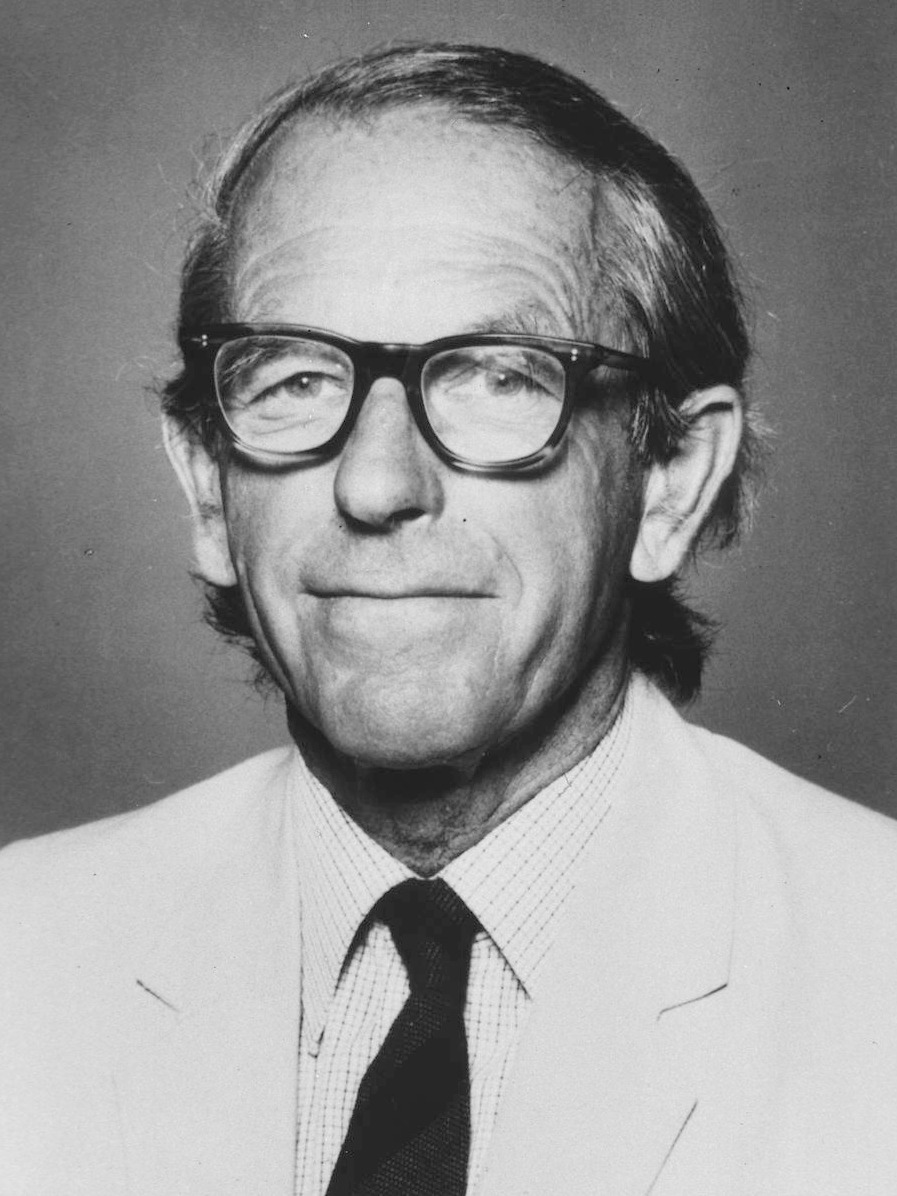
\includegraphics[width=0.30\linewidth]{images/book5/sanger.jpg}\hspace{0.04\linewidth}
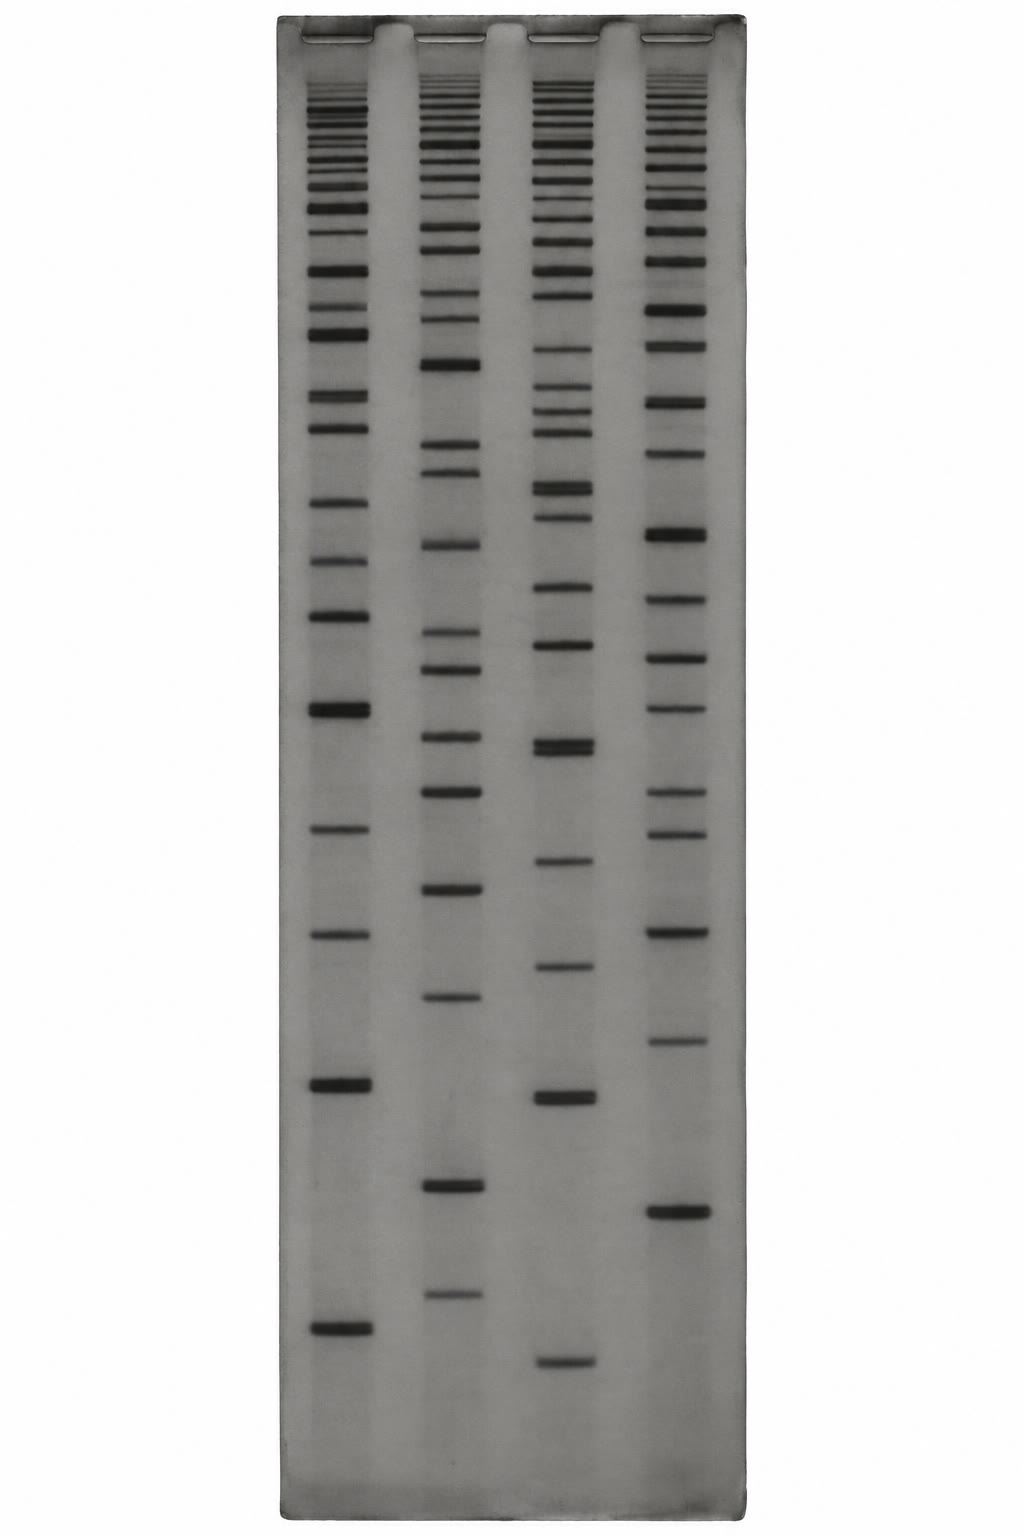
\includegraphics[width=0.30\linewidth]{images/book5/ai/b5-04-sanger-gel.jpg}

{\small Links: Frederick Sanger, die de eerste bruikbare methoden om
eiwitten en DNA te lezen bedacht en voor elk een Nobelprijs kreeg.
Rechts: een autoradiogram van een sequencinggel uit het tijdperk vóór
de capillairen, één baan per base, met de sequentie van onder naar
boven af te lezen uit de ladder van banden.}
\end{omfigure}

\begin{omfigure}
\begin{tikzpicture}[every node/.style={font=\scriptsize}, >=stealth]
  % template and primer
  \draw[very thick, omDef] (0,3.0) -- (6,3.0); \node[left] at (-0.1,3.0) {matrijs 3$'$};
  \node[right] at (6.05,3.0) {5$'$};
  \foreach \x/\b in {0.6/T,1.2/G,1.8/A,2.4/C,3.0/T,3.6/T,4.2/G,4.8/C} \node[above, omDef] at (\x,3.05) {\b};
  \draw[very thick, omProp] (0,2.6) -- (0.3,2.6); \node[left] at (-0.1,2.6) {primer};
  % terminated products
  \foreach \i/\len/\col/\b in {1/0.6/omDef/A, 2/1.2/omMeth/C, 3/1.8/omThm/T, 4/2.4/omExo/G, 5/3.0/omDef/A, 6/3.6/omDef/A, 7/4.2/omMeth/C, 8/4.8/omExo/G} {
    \draw[very thick, omProp] (0,2.6-0.32*\i) -- (\len-0.15,2.6-0.32*\i);
    \fill[\col] (\len-0.05,2.6-0.32*\i) circle (0.1);
    \node[right, \col] at (\len+0.05,2.6-0.32*\i) {dd\b};
  }
  \node[below, align=center] at (2.4,-0.25) {één product voor elke positie, elk eindigend\\op een fluorescerende dideoxybase};
  % capillary readout
  \draw[->, thick] (6.5,1.3) -- (7.4,1.3) node[midway, above] {grootte};
  \draw[thick] (7.6,0.0) rectangle (11.6,2.6);
  \foreach \i/\col in {1/omDef, 2/omMeth, 3/omThm, 4/omExo, 5/omDef, 6/omDef, 7/omMeth, 8/omExo} {
    \draw[very thick, \col] (7.6+0.45*\i,0.1) .. controls (7.6+0.45*\i-0.15,0.1) and (7.6+0.45*\i-0.1,1.6) .. (7.6+0.45*\i,1.6) .. controls (7.6+0.45*\i+0.1,1.6) and (7.6+0.45*\i+0.15,0.1) .. (7.6+0.45*\i+0.3,0.1);
  }
  \foreach \i/\b in {1/A, 2/C, 3/T, 4/G, 5/A, 6/A, 7/C, 8/G} \node[above] at (7.6+0.45*\i,1.7) {\b};
  \node[below] at (9.6,-0.05) {kortste $\to$ langste: de sequentie, in kleur gelezen};
\end{tikzpicture}

{\small Sequencing door \omterm{def:b3:genomics:sanger}{ketenterminatie}. Een dideoxybase beëindigt de
kopie op elke positie waar zij wordt ingebouwd; de fragmenten, één per
lengte, worden op grootte gescheiden en de kleur van elke eindbase
wordt op volgorde afgelezen.}
\end{omfigure}

\begin{definition}[Massaal parallelle sequencing]\label{def:b3:genomics:ngs}
\index{sequencing door synthese}\index{read}\index{sequencing met lange reads}\index{nanoporie}
Instrumenten van de tweede generatie lezen miljoenen tot miljarden
fragmenten tegelijk. Bij \emph{sequencing door synthese} worden de
fragmenten, met adapters aan hun uiteinden geligeerd, aan een glazen
stroomcel gebonden en daar ter plaatse vermenigvuldigd tot clusters
van identieke moleculen; die clusters worden vervolgens per cyclus met
één base verlengd met fluorescerende, omkeerbaar geblokkeerde
nucleotiden, afgebeeld, gedeblokkeerd en opnieuw verlengd, zodat elke
cyclus één base toevoegt aan de \emph{read} van elk cluster. De reads
zijn \qtyrange{100}{300}{bp} lang, meestal vanaf beide uiteinden van
een fragment (\emph{gepaarde uiteinden}), met een foutenpercentage van
ongeveer $10^{-3}$ per base, en één run levert tot $10^{12}$ basen op.
Instrumenten van de derde generatie met \emph{lange reads} lezen
afzonderlijke moleculen zonder vermenigvuldiging: door één polymerase
in reële tijd fluorescerende nucleotiden te zien inbouwen, of door het
DNA door een eiwit-\emph{nanoporie} te rijgen en de ionenstroom te
registreren, die elke opeenvolging van basen op haar eigen manier
moduleert. Reads van \qtyrange{10}{100}{kb} en meer overspannen de
herhalingen waar korte reads niet overheen komen, tegen een hoger ruw
foutenpercentage dat de consensus terugbrengt.
\end{definition}

\begin{omfigure}
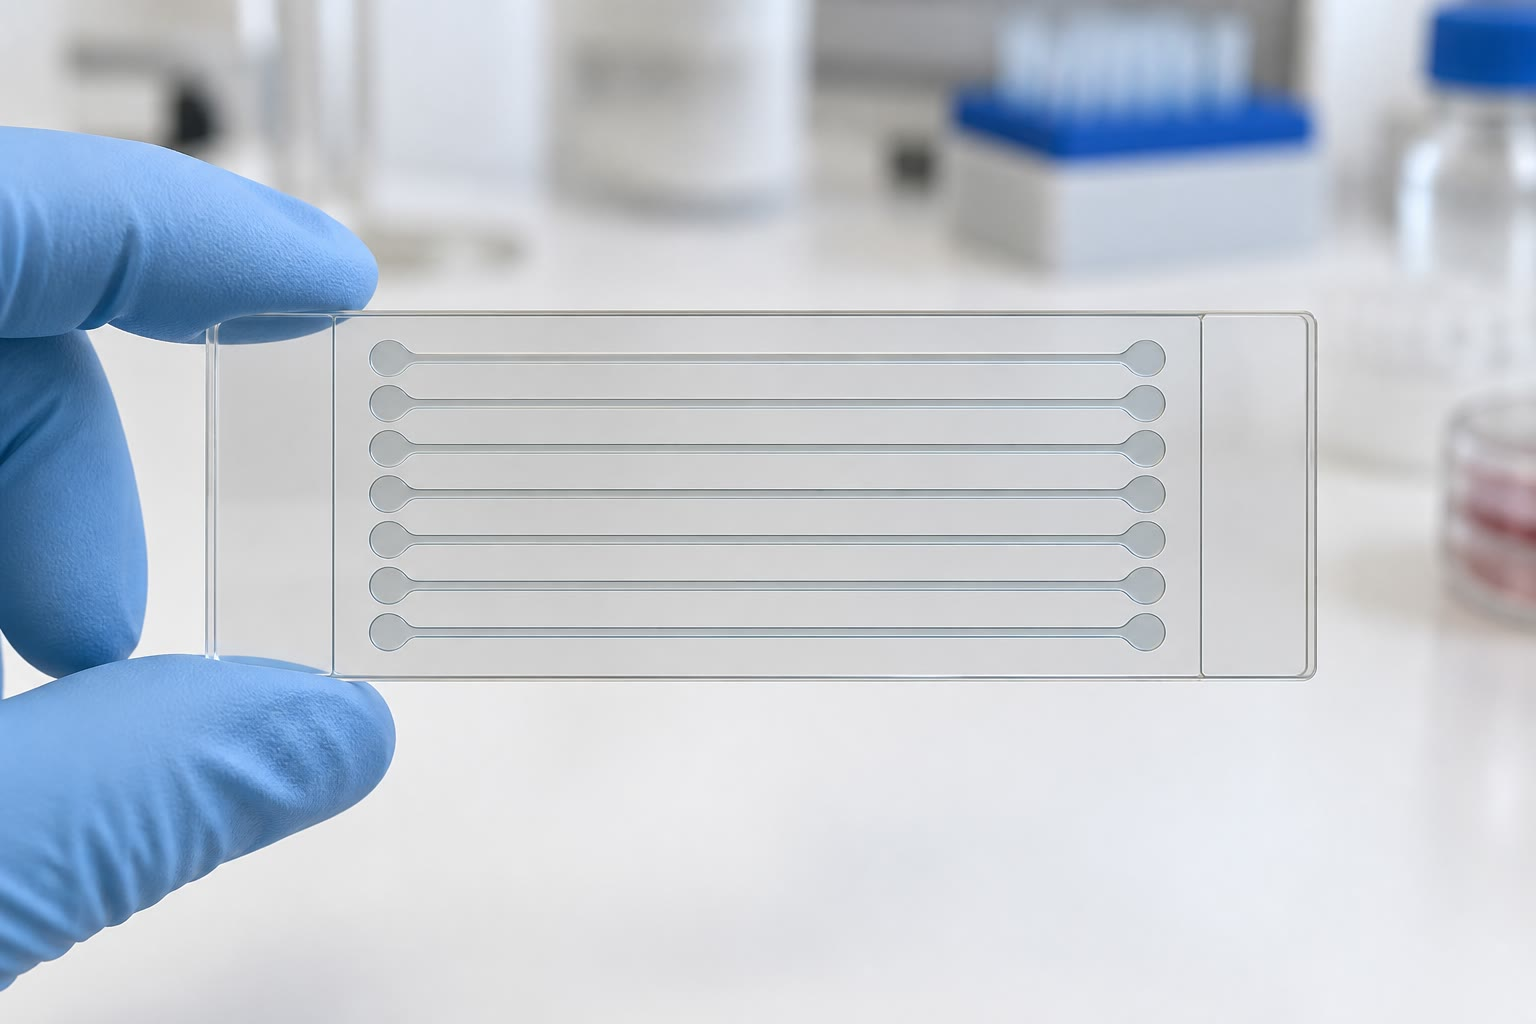
\includegraphics[width=0.46\linewidth]{images/book5/ai/b5-04-flowcell.jpg}\hspace{0.04\linewidth}

\includegraphics[width=0.46\linewidth]{images/book5/ai/b5-04-nanopore.jpg}

{\small Links: een stroomcel, het glazen plaatje waarop miljarden
DNA-clusters worden gekweekt en per cyclus met één base worden
gelezen. Rechts: een nanoporiesequencer ter grootte van een broekzak,
die afzonderlijke moleculen leest als veranderingen in een ionenstroom.}
\end{omfigure}

\begin{theorem}[Dekking en gaten in een hagelschotproject]\label{thm:b3:genomics:lander-waterman}
\index{dekking}\index{Lander--Waterman}\index{contig}
Laat $N$ \omterm{def:b3:genomics:ngs}{reads} van lengte $L$ op willekeurige posities langs een genoom
van lengte $G$ worden genomen, en zij $c = NL/G$ de \emph{dekking}, het
gemiddelde aantal \omterm{def:b3:genomics:ngs}{reads} dat een base bedekt. Dan wordt een gegeven base
bedekt door een aantal \omterm{def:b3:genomics:ngs}{reads} dat poissonverdeeld is met gemiddelde $c$:
het deel van het genoom dat ongesequenced blijft is
\[
P(\text{onbedekt}) = e^{-c},
\]
en als twee \omterm{def:b3:genomics:ngs}{reads} pas als overlappend worden herkend wanneer zij
minstens $T$ basen delen, zodat $\theta = T/L$, is het verwachte aantal
\emph{contigs} (eilanden van overlappende \omterm{def:b3:genomics:ngs}{reads})
\[
\text{contigs} = N\,e^{-c(1-\theta)},
\]
en hun gemiddelde lengte is bij benadering
$L\,\bigl(e^{c(1-\theta)} - 1\bigr)/c + L\theta$.
\end{theorem}
\begin{proof}
De beginpunten van de \omterm{def:b3:genomics:ngs}{reads} vallen willekeurig met dichtheid $N/G$ per
base. Een base wordt bedekt door de \omterm{def:b3:genomics:ngs}{reads} die in de $L$ basen ervóór
beginnen; het aantal beginpunten in een venster van lengte $L$ is
poissonverdeeld met gemiddelde $LN/G
= c$, en de kans op geen enkel beginpunt is $e^{-c}$. Een \omterm{def:b3:genomics:ngs}{read} is de
meest rechtse van zijn contig als geen andere \omterm{def:b3:genomics:ngs}{read} begint binnen de
$L - T = L(1-\theta)$ basen na zijn eigen beginpunt (een \omterm{def:b3:genomics:ngs}{read} die later
begint zou hem met minder dan $T$ overlappen en niet worden
aangehecht); die kans is $e^{-c(1-\theta)}$, en omdat elke contig
precies één meest rechtse \omterm{def:b3:genomics:ngs}{read} heeft, is het verwachte aantal contigs
$N e^{-c(1-\theta)}$. De gemiddelde contiglengte volgt uit $G$ gedeeld
door het aantal contigs, gecorrigeerd voor het onbedekte deel.
\end{proof}

\begin{example}[Hoeveel genoeg is]\label{ex:b3:genomics:coverage}
Bij $c = 5$ is het ongesequencede deel $e^{-5} = 0.7\,\%$ --- voor een
genoom van \qty{3.2}{Gb} twintig miljoen basen in enkele tienduizenden
gaten. Bij $c = 10$ is het $4.5\times 10^{-5}$, in totaal
\qty{150}{kb}. Menselijke genomen worden standaard bij $c = 30$
gesequenced, niet vanwege dekkingsgaten ($e^{-30} \approx 10^{-13}$)
maar omdat elke base op elk van de twee chromosomen meermalen moet
worden gelezen om een heterozygote variant met vertrouwen vast te
stellen tegen een foutenpercentage van $10^{-3}$ per \omterm{def:b3:genomics:ngs}{read}. Bacteriële
genomen worden bij $c = 50$--$100$ gesequenced om dezelfde reden en
omdat het goedkoop is. De formule laat ook zien wat dekking niet kan
oplossen: een herhaling die langer is dan een \omterm{def:b3:genomics:ngs}{read} is een plaats waar
de overlapgraaf zich vertakt, en geen enkele hoeveelheid korte \omterm{def:b3:genomics:ngs}{reads}
lost dat op. Daar zijn lange \omterm{def:b3:genomics:ngs}{reads} voor.
\end{example}

\begin{omfigure}
\begin{tikzpicture}
\begin{axis}[
  width=0.7\linewidth, height=5.6cm,
  axis x line=bottom, axis y line=left,
  xmin=0, xmax=12, ymin=0.000001, ymax=1, ymode=log,
  xlabel={dekking $c$}, ylabel={fractie},
  xlabel style={font=\small, at={(axis description cs:0.5,-0.12)}, anchor=north},
  ylabel style={font=\small},
  tick label style={font=\small}, xtick={0,2,4,6,8,10,12},
  clip=false,
]
\addplot[very thick, omDef, domain=0:12, samples=40] {exp(-x)};
\addplot[very thick, omThm, domain=0.3:12, samples=40] {exp(-x*0.8)*x/12};
\node[font=\scriptsize, omDef, anchor=north west] at (axis cs:0.3,0.002) {onbedekt deel $e^{-c}$};
\node[font=\scriptsize, omThm, anchor=south west] at (axis cs:5.5,0.03) {contigs per read $\times\, c/12$, $\theta = 0.2$};
\end{axis}
\end{tikzpicture}

{\small De twee grootheden van Lander--Waterman tegen de dekking: het
deel van het genoom dat nooit wordt gelezen daalt als $e^{-c}$, en het
aantal contigs (hier per \omterm{def:b3:genomics:ngs}{read} geschaald) bereikt bij lage dekking een
maximum en daalt daarna terwijl de eilanden samensmelten.}
\end{omfigure}

\section{Van reads naar een genoom}

\begin{definition}[Assemblage en annotatie]\label{def:b3:genomics:assembly}
\index{assemblage}\index{scaffold}\index{N50}\index{annotatie}\index{referentiegenoom}
De \emph{assemblage} reconstrueert een genoom uit zijn \omterm{def:b3:genomics:ngs}{reads} via
overlap: in een \emph{overlapgraaf} is elke \omterm{def:b3:genomics:ngs}{read} een knoop, verbonden
met de \omterm{def:b3:genomics:ngs}{reads} die hij overlapt; in een \emph{De Bruijn-graaf}, gebruikt
voor miljarden korte \omterm{def:b3:genomics:ngs}{reads}, is elke $k$-meer (deelsequentie van lengte
$k$) een knoop en is het genoom een pad erdoorheen. Beide worden
gebroken door herhalingen die langer zijn dan de \omterm{def:b3:genomics:ngs}{read}, die vertakkende
paden geven. Contigs worden door gepaarde \omterm{def:b3:genomics:ngs}{reads} en informatie over
grote afstand (lange \omterm{def:b3:genomics:ngs}{reads}, optische kaarten, kaarten van
chromosoomcontacten) geordend en gericht tot \emph{scaffolds}, en de
scaffolds worden op de chromosomen geplaatst. De kwaliteit van een
assemblage wordt samengevat door de \emph{N50}: de contiglengte
waarvoor de helft van de geassembleerde basen in contigs van minstens
die lengte ligt. De \emph{annotatie} zoekt daarna de genen: bij
bacteriën open leesramen die langer zijn dan het toeval geeft; bij
eukaryoten door sequentiesignalen (splitsplaatsen, promotoren,
codonvoorkeur), homologie met bekende eiwitten en uit RNA gesequencede
transcripten te combineren. Het resultaat is voor een soort een
\emph{referentiegenoom} waartegen elke latere \omterm{def:b3:genomics:ngs}{read} van die soort wordt
uitgelijnd in plaats van opnieuw geassembleerd.
\end{definition}

\begin{method}[Van een monster naar varianten]\label{met:b3:genomics:pipeline}
\index{variantbepaling}
Voor een studie waarin een individu opnieuw wordt gesequenced tegen een
referentie: (1) haal het DNA eruit, fragmenteer het tot
\qtyrange{300}{500}{bp} en ligeer er adapters aan (de
\emph{bibliotheek}); (2) sequenceer tot de vereiste dekking
(30$\times$ voor een menselijk genoom, 100$\times$ voor een exoom, dat
de \qty{1.5}{\%} van het genoom vangt die voor eiwit codeert); (3) lijn
elke \omterm{def:b3:genomics:ngs}{read} uit tegen de referentie, met tolerantie voor mismatches;
(4) tel op elke positie de basen in de \omterm{def:b3:genomics:ngs}{reads}: een positie waar ongeveer
de helft van de \omterm{def:b3:genomics:ngs}{reads} van de referentie afwijkt is een heterozygote
\emph{variant}, waar vrijwel alle \omterm{def:b3:genomics:ngs}{reads} afwijken een homozygote, en
waar enkele \omterm{def:b3:genomics:ngs}{reads} afwijken een fout; (5) filter op diepte,
basekwaliteit en strengbalans; (6) annoteer elke variant met haar
effect op een gen (synoniem, missense, nonsense, splitsplaats,
leesraamverschuiving) en met haar frequentie in populatiedatabanken;
(7) houd voor een diagnose de zeldzame varianten over die schadelijk
worden voorspeld in genen die bij het fenotype passen, en bevestig ze
met \omterm{def:b3:genomics:sanger}{Sanger-sequencing}.
\end{method}

\section{Hoe genomen eruitzien}

\begin{proposition}[Genoomgrootte en aantal genen]\label{prop:b3:genomics:sizes}
\index{C-waardeparadox}\index{genoomgrootte}
\omterm{prop:b3:genomics:sizes}{Genoomgroottes} beslaan bij eukaryoten een factor $10^{5}$ ---
\qty{12}{Mb} voor gist, \qty{100}{Mb} voor de worm, \qty{140}{Mb} voor
de vlieg, \qty{3.2}{Gb} voor een mens, \qty{16}{Gb} voor een ui,
\qty{130}{Gb} voor een longvis, \qty{150}{Gb} voor de lelie \emph{Paris
japonica} --- terwijl de aantallen genen amper een factor $10$
beslaan: \num{6000} bij gist, \num{20000} bij de worm, \num{14000} bij
de vlieg, ongeveer \num{20000} eiwitcoderende genen bij een mens,
\num{40000} bij rijst. Dat is de \emph{C-waardeparadox}: de
\omterm{prop:b3:genomics:sizes}{genoomgrootte} meet de complexiteit niet, en het aantal genen evenmin.
Wat varieert is de niet-coderende inhoud --- introns, verplaatsbare
elementen, satellietherhalingen --- en het aantal eiwitten dat een
genoom kan voortbrengen wordt ver boven zijn aantal genen
vermenigvuldigd door alternatieve splicing
(\cref{ch:b3:rna-regulation}) en door regulatie, en daar is de
complexiteit van een organisme grotendeels geschreven. Bacteriële
genomen zijn daarentegen compact en hun grootte volgt het aantal genen
wel: ongeveer één gen per kilobase, \qty{88}{\%} coderend bij
\emph{E.~coli}.
\end{proposition}

\begin{example}[Het menselijk genoom naar inhoud]\label{ex:b3:genomics:content}
Van de \qty{3.2}{Gb}: eiwitcoderende exons \qty{1.5}{\%}; introns en
niet-vertaalde regio's van genen ongeveer \qty{35}{\%}; verplaatsbare
elementen en hun fossielen ongeveer \qty{45}{\%} ---
LINE-1-retrotransposons \qty{17}{\%}, Alu-elementen \qty{10}{\%} (ruim
een miljoen kopieën van een sequentie van \qty{300}{bp}), endogene
retrovirussen \qty{8}{\%}; segmentale duplicaties \qty{5}{\%};
eenvoudige herhalingen en satellieten, met inbegrip van de centromeren,
ongeveer \qty{5}{\%}; de rest unieke niet-coderende sequentie, waar de
regulerende elementen wonen. Zo'n \numrange{100}{200} genen coderen nog
voor werkzame LINE-1-machinerie, en nieuwe inserties treden ongeveer
eens per twintig geboorten op. Ongeveer \qty{8}{\%} van het genoom
staat onder aantoonbare zuiverende selectie --- veel meer dan de exons
--- en het meeste daarvan is regulerend.
\end{example}

\begin{omfigure}
\begin{tikzpicture}[every node/.style={font=\scriptsize}]
  \def\w{12}
  % stacked bar: fractions
  \fill[omThm] (0,0) rectangle (0.18,0.7);
  \fill[omDef!60] (0.18,0) rectangle (4.38,0.7);
  \fill[omProp!70] (4.38,0) rectangle (6.42,0.7);
  \fill[omProp!45] (6.42,0) rectangle (7.62,0.7);
  \fill[omProp!25] (7.62,0) rectangle (9.78,0.7);
  \fill[omMeth!50] (9.78,0) rectangle (10.38,0.7);
  \fill[gray!45] (10.38,0) rectangle (10.98,0.7);
  \fill[gray!15] (10.98,0) rectangle (12,0.7);
  \draw[thick] (0,0) rectangle (12,0.7);
  % labels above/below with leaders
  \draw (0.09,0.7) -- (0.09,1.1); \node[above, align=center] at (0.5,1.1) {exons\\\qty{1.5}{\%}};
  \node[above] at (2.3,0.75) {introns en UTR's van genen: \qty{35}{\%}};
  \node[below, align=center] at (5.4,-0.05) {LINE-1\\\qty{17}{\%}};
  \node[below, align=center] at (7.0,-0.05) {Alu\\\qty{10}{\%}};
  \node[below, align=center] at (8.7,-0.05) {overige transposons,\\retrovirussen \qty{18}{\%}};
  \node[above, align=center] at (10.1,0.75) {segmentale\\duplicaties \qty{5}{\%}};
  \node[below, align=center] at (10.7,-0.05) {satellieten\\\qty{5}{\%}};
  \draw[gray] (11.5,0.72) -- (12.0,1.05); \node[above, align=center] at (12.3,1.05) {overige unieke\\niet-coderende};
  \draw[decorate, decoration={brace, amplitude=4pt, mirror}] (4.38,-1.0) -- (9.78,-1.0) node[midway, below=4pt] {afgeleid van verplaatsbare elementen: \qty{45}{\%}};
\end{tikzpicture}

{\small Het menselijk genoom naar inhoud, op schaal. De eiwitcoderende
exons (rood) zijn een splinter; bijna de helft van het genoom stamt af
van verplaatsbare elementen.}
\end{omfigure}

\begin{definition}[Vergelijkende genomica]\label{def:b3:genomics:comparative}
\index{ortholoog}\index{paraloog}\index{syntenie}\index{geconserveerd niet-coderend element}\index{volledige-genoomduplicatie}
Genen in twee soorten die van één gen in hun gemeenschappelijke
voorouder afstammen zijn \emph{orthologen}; genen binnen één soort die
van een duplicatie afstammen zijn \emph{paralogen}. Blokken chromosoom
waarin de genvolgorde tussen soorten bewaard is gebleven zijn
\emph{synteen}; syntenie laat een gen in het ene genoom opsporen vanuit
zijn positie in het andere en legt de herschikkingen bloot die twee
karyotypen scheiden (ongeveer \num{1000} tussen mens en muis).
Sequenties die over verre soorten heen zijn geconserveerd en voor geen
eiwit coderen --- \emph{geconserveerde niet-coderende elementen},
waarvan sommige over \qty{200}{bp} tussen mens en vis tot op de base
ultrageconserveerd zijn --- zijn meestal enhancers van
ontwikkelingsgenen. \emph{Volledige-genoomduplicaties} hebben de
geschiedenis van afstammingslijnen getekend: twee ronden aan de
oorsprong van de gewervelden (de vier Hox-clusters van zoogdieren tegen
de ene van ongewervelden), één in de voorouder van de zalmachtigen, één
in de gistlijn, verscheidene bij bloemplanten; de dubbele genen gaan
over tientallen miljoenen jaren grotendeels verloren, en de
overlevenden lopen in functie uiteen.
\end{definition}

\begin{example}[Mens en chimpansee]\label{ex:b3:genomics:chimp}
Uitgelijnde enkelvoudige sequentie verschilt tussen mens en chimpansee
in \qty{1.2}{\%} van de basen --- zo'n \num{35} miljoen substituties
--- en door inserties en deleties die samen nog eens \qty{3}{\%} van
elk genoom beslaan. Twee mensen verschillen op ongeveer één base op
duizend, zo'n \numrange{4}{5} miljoen plaatsen, plus enkele duizenden
structurele varianten; twee chimpansees, waarvan de populatie langer
groter is geweest, op nogal wat meer. Een kind draagt ongeveer \num{70}
nieuwe mutaties die bij beide ouders ontbreken, vier vijfde daarvan van
de vader, en het aantal stijgt met ongeveer twee per jaar
vaderleeftijd --- de rekensom van \cref{ch:b3:dna-repair} toegepast op
de vele delingen van de spermatogenese.
\end{example}

\section{Genomen en eigenschappen}

\begin{definition}[Genoombrede associatie]\label{def:b3:genomics:gwas}
\index{genoombrede associatiestudie}\index{enkelnucleotidepolymorfisme}\index{polygene score}
Een \emph{enkelnucleotidepolymorfisme} (SNP) is een positie waar twee
basen elk bij minstens \qty{1}{\%} van een populatie voorkomen; bij de
mens zijn er ongeveer tien miljoen algemeen. Een \emph{genoombrede
associatiestudie} (GWAS) bepaalt het genotype van honderdduizenden
SNP's bij duizenden mensen met een ziekte en duizenden zonder, en
vraagt bij elke SNP of het ene allel vaker bij de gevallen voorkomt.
Omdat er een miljoen toetsen worden uitgevoerd, telt een uitkomst pas
onder een significantiedrempel van ongeveer $5\times 10^{-8}$ ($0.05$
gedeeld door de miljoen feitelijk onafhankelijke toetsen).
Geassocieerde SNP's markeren een gebied, niet een oorzakelijke
variant, omdat naburige allelen samen reizen
(koppelingsonevenwicht) over tientallen kilobasen. Bij de meeste
veelvoorkomende ziekten verschuift elk geassocieerd allel het risico
met enkele procenten en ligt het meestal in regulerende sequentie; hun
gezamenlijke effect, over duizenden SNP's opgeteld als een
\emph{polygene score}, verklaart een deel van de erfelijkheid en
voorspelt het risico ongeveer even goed als de familiegeschiedenis.
\end{definition}

\begin{remark}[Wat de genomica wel en niet heeft gebracht]\label{rem:b3:genomics:delivered}
Sequencing is doorslaggevend geweest waar één gen een groot effect
heeft: enkele duizenden mendeliaanse ziekten hebben hun gen, en het
sequencen van het exoom van een kind met een niet-gediagnosticeerde
aandoening levert in ongeveer een derde van de gevallen een diagnose
op. Tumorgenomen laten zien welke aandrijvers een tumor draagt en welke
middelen kunnen werken (\cref{ch:b3:cancer-biology});
ziekteverwekkergenomen volgen uitbraken stam voor stam
(\cref{ch:b3:bacteriology}); oude genomen hebben de menselijke
voorgeschiedenis herschreven en laten zien dat mensen buiten Afrika
ongeveer \qty{2}{\%} neanderthaler-DNA dragen. Voor veelvoorkomende
ziekten --- diabetes, hartziekte, schizofrenie --- heeft de genomica
duizenden kleine effecten en weinig mechanismen opgeleverd, en de
belofte van voorspelling uit een genoom van een gezond mens blijft
bescheiden. Het genoom is een onderdelenlijst; de biologie van hoe de
onderdelen samenwerken is er niet uit af te lezen.
\end{remark}

\section{Opgaven}

\begin{exercise}[$\star$]\label{exo:b3:genomics:1}
Leg uit waarom een \omterm{def:b3:genomics:sanger}{dideoxynucleotide} een groeiende DNA-keten beëindigt,
en waarom een Sanger-reactie van elk nucleotide zowel de normale als de
dideoxyvorm moet bevatten.
\end{exercise}

\begin{exercise}[$\star$]\label{exo:b3:genomics:2}
Eén run levert $4\times 10^{8}$ gepaarde \omterm{def:b3:genomics:ngs}{reads} van
$2\times \qty{150}{bp}$. Welke dekking geeft dat van een menselijk
genoom van \qty{3.2}{Gb}? En van een bacterieel genoom van \qty{5}{Mb}?
\end{exercise}

\begin{exercise}[$\star$]\label{exo:b3:genomics:3}
Definieer contig, \omterm{def:b3:genomics:assembly}{scaffold} en \omterm{def:b3:genomics:assembly}{N50}. Een \omterm{def:b3:genomics:assembly}{assemblage} van \qty{100}{Mb}
heeft tien contigs van \qty{8}{Mb} en \num{2000} van \qty{10}{kb}. Wat
is haar \omterm{def:b3:genomics:assembly}{N50}?
\end{exercise}

\begin{exercise}[$\star$]\label{exo:b3:genomics:4}
Formuleer de C-waardeparadox met twee voorbeelden, en zeg waaruit het
overtollige DNA van grote genomen vooral bestaat.
\end{exercise}

\begin{exercise}[$\star\star$]\label{exo:b3:genomics:5}
Bepaal met \cref{thm:b3:genomics:lander-waterman} de dekking die nodig
is om hoogstens één base op een miljoen ongesequenced te laten, en het
verwachte aantal contigs voor een genoom van \qty{5}{Mb} dat bij
$c = 8$ wordt gelezen met \omterm{def:b3:genomics:ngs}{reads} van \qty{150}{bp} en een minimale
overlap van \qty{30}{bp}.
\end{exercise}

\begin{exercise}[$\star\star$]\label{exo:b3:genomics:6}
Een heterozygote variant wordt door $30$ \omterm{def:b3:genomics:ngs}{reads} bedekt. Wat is, als elke
\omterm{def:b3:genomics:ngs}{read} met kans $1/2$ het ene of het andere allel toont, de kans dat
minder dan $8$ \omterm{def:b3:genomics:ngs}{reads} het variante allel tonen (zodat het voor fouten
zou kunnen worden aangezien)? Gebruik een normale benadering met
gemiddelde $15$ en standaardafwijking $\sqrt{7.5}$. Waarom is
$30\times$ de standaard?
\end{exercise}

\begin{exercise}[$\star\star$]\label{exo:b3:genomics:7}
Een genoom bevat een herhaling van \qty{6}{kb} in \num{500} kopieën.
Leg uit waarom een \omterm{def:b3:genomics:assembly}{assemblage} uit \omterm{def:b3:genomics:ngs}{reads} van \qty{150}{bp} haar laat
inklappen, hoe de resulterende graaf eruitziet, en welke readlengte
haar zou oplossen.
\end{exercise}

\begin{exercise}[$\star\star$]\label{exo:b3:genomics:8}
Twee mensen verschillen op één base op duizend. Hoeveel verschillen
zitten er in hun exomen (\qty{48}{Mb} coderende sequentie)? Als twee
derde van de coderende verschillen synoniem of onschadelijk is en de
rest een eiwit verandert, hoeveel eiwitveranderende varianten draagt de
ene persoon dan ten opzichte van de andere?
\end{exercise}

\begin{exercise}[$\star\star$]\label{exo:b3:genomics:9}
Een GWAS toetst $10^{6}$ SNP's bij drempel $p < 5\times 10^{-8}$.
Hoeveel valse positieven zijn er te verwachten als geen enkele SNP echt
geassocieerd is? Een SNP-allel verhoogt het risico op een ziekte met
frequentie \qty{2}{\%} naar \qty{2.3}{\%}. Leg uit waarom zo'n effect
in een studie met duizend mensen niet aantoonbaar is en voor een
individu nutteloos, en toch naar een mechanisme kan wijzen.
\end{exercise}

\begin{exercise}[$\star\star\star$]\label{exo:b3:genomics:10}
Bacteriële genomen zijn voor ongeveer \qty{88}{\%} coderend, het
menselijk genoom voor \qty{1.5}{\%}. Geef drie hypothesen ---
populatiegenetisch, structureel en regulerend --- voor het verschil, en
bij elk een waarneming aan genomen die haar steunt of ondergraaft.
\end{exercise}

\begin{exercise}[$\star\star\star$]\label{exo:b3:genomics:11}
Leid de contigtelling van Lander--Waterman af voor een mengsel van
\omterm{def:b3:genomics:ngs}{reads} van twee lengtes: $N_{1}$ korte \omterm{def:b3:genomics:ngs}{reads} van lengte $L_{1}$ en
$N_{2}$ lange \omterm{def:b3:genomics:ngs}{reads} van lengte $L_{2}$, met overlappen die met dezelfde
minimale $T$ worden geteld. (Beschouw elke \omterm{def:b3:genomics:ngs}{read} als de meest rechtse
van zijn contig als er geen \omterm{def:b3:genomics:ngs}{read} van welke soort dan ook begint binnen
zijn eigen lengte min $T$.) Laat zien dat enkele lange \omterm{def:b3:genomics:ngs}{reads} de
contigtelling meer verlagen dan hetzelfde aantal basen in korte \omterm{def:b3:genomics:ngs}{reads}.
\end{exercise}

\begin{exercise}[$\star\star\star$]\label{exo:b3:genomics:12}
Van de vier Hox-clusters van zoogdieren wordt betoogd dat zij door twee
ronden van \omterm{def:b3:genomics:comparative}{volledige-genoomduplicatie} aan de basis van de gewervelden
uit één cluster afstammen. Zeg welk patroon van paralogen door het
genoom heen, en welk patroon in de genomen van prikken en van de
ongewervelde chordaten, die hypothese voorspelt, en hoe men haar zou
onderscheiden van twee onafhankelijke duplicaties van alleen het
cluster.
\end{exercise}

\section{Vraagstuk: twee genomen op één machine}

\begin{problem}[{Weekendvraagstuk --- een bacterie en een mens
gesequenced op dezelfde run: de reads verdeeld, de dekking en de gaten
berekend, de contigs geteld, de heterozygote varianten bepaald tegen
het foutenpercentage, de inhoud van het menselijk genoom gewogen en een
associatiestudie op maat gemaakt, met als besluit de contigtelling bij
lage dekking, de dekking die een variantbepaling veilig maakt en het
aantal nieuwe mutaties bij een kind}]
\label{pb:b3:genomics:1}
Gegevens: één run levert $6\times 10^{8}$ \omterm{def:b3:genomics:ngs}{reads} van \qty{150}{bp}. Een
bacterieel genoom is \qty{4.6}{Mb}; het menselijk genoom \qty{3.2}{Gb}
(haploïd). Minimale overlap $T = \qty{30}{bp}$. Foutenpercentage
$10^{-3}$ per base per \omterm{def:b3:genomics:ngs}{read}. Menselijke coderende sequentie
\qty{48}{Mb}; het genoom is voor \qty{45}{\%} van transposons afgeleid,
met $1.1$ miljoen Alu-kopieën van \qty{300}{bp}. Twee mensen
verschillen op één plaats op \num{1000}. Mutatiesnelheid
$1.2\times 10^{-8}$ per base per generatie.

\medskip
\noindent\textbf{Deel I --- De bacterie.}
\begin{enumerate}
  \item De bacterie krijgt \qty{0.2}{\%} van de run. Hoeveel \omterm{def:b3:genomics:ngs}{reads}, en
        welke dekking?
  \item Welk deel van haar genoom blijft ongesequenced? Hoeveel basen
        zijn dat?
  \item Bereken $\theta$ en het verwachte aantal contigs.
  \item Een eerdere proefrun gebruikte maar \num{30000} \omterm{def:b3:genomics:ngs}{reads}. Dekking,
        onbedekt deel en aantal contigs?
  \item Het genoom bevat \num{7} kopieën van een rRNA-operon van
        \qty{5}{kb}. Leg uit wat er in de \omterm{def:b3:genomics:assembly}{assemblage} met hen gebeurt en
        hoeveel contiguiteinden dit alleen al oplevert.
  \item De bacterie heeft ongeveer één gen per kilobase. Hoeveel genen,
        en, als \qty{88}{\%} van het genoom coderend is, wat is de
        gemiddelde genlengte?
\end{enumerate}

\medskip
\noindent\textbf{Deel II --- De mens.}
\begin{enumerate}[resume]
  \item De rest van de run gaat naar één menselijk genoom. Welke
        dekking van het diploïde genoom per haploïde kopie (dat wil
        zeggen het totaal aantal basen gedeeld door \qty{3.2}{Gb})?
  \item Op een heterozygote plaats wordt elk van de twee allelen door
        ongeveer de helft van de \omterm{def:b3:genomics:ngs}{reads} bedekt. Wat is met de dekking uit
        vraag 7 het verwachte aantal \omterm{def:b3:genomics:ngs}{reads} dat elk allel toont?
  \item Een fout toont met kans $10^{-3}$ een verkeerde base in een
        \omterm{def:b3:genomics:ngs}{read}. Wat is op een homozygote plaats die door $c$ \omterm{def:b3:genomics:ngs}{reads} wordt
        bedekt het verwachte aantal \omterm{def:b3:genomics:ngs}{reads} dat een bepaalde verkeerde
        base toont (elk $10^{-3}/3$)? Waarom verwerpt een regel ``bepaal
        een variant als minstens $3$ \omterm{def:b3:genomics:ngs}{reads} en minstens \qty{20}{\%} van
        de \omterm{def:b3:genomics:ngs}{reads} haar tonen'' bij deze dekking de fouten?
  \item Hoeveel heterozygote plaatsen draagt één mens (ruwweg de helft
        van de verschillen tussen twee willekeurige genomen ligt in
        elk: neem één plaats op \num{1500})? Hoeveel in coderende
        sequentie?
  \item De \omterm{def:b3:genomics:ngs}{reads} worden tegen een referentie uitgelijnd. Leg uit waarom
        \omterm{def:b3:genomics:ngs}{reads} uit Alu-elementen vaak op de verkeerde kopie terechtkomen
        en welk gevolg dat heeft voor het bepalen van varianten erin.
  \item Een kind wordt samen met beide ouders gesequenced. Hoeveel
        nieuwe mutaties zijn er te verwachten? Hoeveel \omterm{def:b3:genomics:ngs}{reads} bij het
        kind moeten bij deze dekking een variant tonen die bij
        \emph{beide} ouders ontbreekt voordat men haar gelooft, en
        waarom is de dekking bij de ouders even belangrijk als die bij
        het kind?
  \item Een klinisch laboratorium vangt het exoom (\qty{48}{Mb}) en
        sequenceert het bij $100\times$. Hoeveel \omterm{def:b3:genomics:ngs}{reads} kost dat, en
        waarom is het per patiënt goedkoper dan een genoom bij
        $28\times$, hoewel de dekking hoger is?
\end{enumerate}

\medskip
\noindent\textbf{Deel III --- De inhoud van een genoom.}
\begin{enumerate}[resume]
  \item Welk deel van het menselijk genoom is Alu, en welk deel van de
        \omterm{def:b3:genomics:ngs}{reads} uit vraag 7 komt uit Alu-elementen?
  \item De referentie is \qty{3.2}{Gb} maar een diploïde cel bevat
        \qty{6.4}{Gb}; en een ui van \qty{16}{Gb} heeft ongeveer
        \num{60000} genen. Wat is het coderende deel van het
        uiengenoom, als zijn genen gemiddeld \qty{1.5}{kb} coderende
        sequentie hebben?
  \item Mens en chimpansee verschillen op \qty{1.2}{\%} van de
        uitgelijnde basen. Hoeveel substituties zijn dat in
        \qty{2.9}{Gb} uitlijnbare sequentie? Welke mutatiesnelheid per
        base per jaar volgt hieruit als zij gelijk over de twee
        afstammingslijnen worden verdeeld over $6.5$ miljoen jaar, en
        welke per generatie van $25$ jaar? Vergelijk met de
        rechtstreekse meting uit de gegevens.
  \item Twee genoomduplicaties bij de gewervelden zouden tot vier
        kopieën van elk voorouderlijk gen moeten geven. Mensen hebben
        ongeveer \num{20000} genen en de ongewervelde chordaat
        \emph{Ciona} ongeveer \num{16000}. Welk deel van de duplicaten
        is verloren gegaan, onder de hypothese dat de voorouder er
        \num{16000} had?
  \item Leg uit waarom het aantal genen een slechte maat voor de
        complexiteit van een organisme is, met de telling van de
        alternatieve splicing uit \cref{ch:b3:rna-regulation} als één
        argument.
  \item \qty{8}{\%} van het genoom staat onder zuiverende selectie maar
        slechts \qty{1.5}{\%} codeert voor eiwit. Wat is de rest
        waarschijnlijk, en hoe zou één kandidaat-element te toetsen
        zijn?
\end{enumerate}

\medskip
\noindent\textbf{Deel IV --- Een associatiestudie.}
\begin{enumerate}[resume]
  \item Er worden $10^{6}$ SNP's getoetst. Geef de bonferronidrempel
        voor een gezinsgewijze fout van $0.05$, en het verwachte aantal
        valse positieven bij $p < 10^{-5}$.
  \item Een ziekte heeft een prevalentie van \qty{1}{\%}. Een
        risicoallel met frequentie $0.3$ verhoogt de odds met
        \qty{5}{\%}. Bereken het ziekterisico van een drager van twee
        kopieën, van één kopie en van geen enkele, met \qty{0.9}{\%}
        als risico voor een niet-drager. (Vermenigvuldig de odds.)
  \item Er worden tweehonderd zulke allelen gevonden. Leg uit wat een
        \omterm{def:b3:genomics:gwas}{polygene score} is, en waarom de score van iemand in de bovenste
        \qty{1}{\%} met een meervoudig risico kan overeenkomen hoewel
        elk allel vrijwel niets doet.
  \item Leg uit waarom een SNP die significantie bereikt meestal niet de
        oorzakelijke variant is, en welk experiment de oorzakelijke in
        het gebied zou aanwijzen.
  \item Een oud genoom uit een bot van \num{40000} jaar oud wordt bij
        $c = 0.5$ gesequenced. Welk deel ervan wordt gelezen? Waarom kan
        dit toch vragen over de geschiedenis van populaties
        beantwoorden die een modern genoom alleen niet kan?
  \item Vat samen: het aantal contigs in de proefassemblage (vraag~4),
        de dekking per haploïd genoom die ongeveer $15$ \omterm{def:b3:genomics:ngs}{reads} per allel
        geeft (vraag~7--8), en het aantal nieuwe mutaties bij een kind
        (vraag~12).
\end{enumerate}
\end{problem}
